\documentclass{article}

\usepackage[margin=1in]{geometry}
\usepackage{graphicx}
\usepackage{enumitem}
\usepackage{parskip}

\title{Von Neumann Standing -- Official documentation}
\date{\today}
\author{Louis A. Burke}

\begin{document}
\maketitle \clearpage

\section*{Motivation}

The goal of this game is to write the most efficient code to defeat your
opponent. Everything from cache misses to branch prediction failures will
contribute to your units' reaction times.

\section*{Summary}

Control your squad of robotic soldiers to defeat your opponent!

Each team starts with the following units:

\begin{itemize}[noitemsep]
    \item[$\bullet$] Captain
    \item[$\bullet$] Mortar
    \item[$\bullet$] Sniper
    \item[$\bullet\bullet$] Engineer
    \item[$\bullet\bullet$] Machinegunner
    \item[$\bullet\bullet$] Scout
    \item[$\bullet\bullet$] Rifleman
\end{itemize}

Additionally each unit has the following stats:

\begin{itemize}[noitemsep]
    \item[$\bullet$] Cache Size
    \item[$\bullet$] Cache Type
    \item[$\bullet$] Branch Predictors
    \item[$\bullet$] Clock
\end{itemize}

Each unit runs its own code. Units can communicate via shared pools of memory.
This represents their communication link. For example the captain has
communication with all units, but not all other unit pairs have direct
communication.

Every frame each team gains one resource point. These points can be spent on
upgrades and munitions for your units.

\section*{Rules}

Each player must write 11 programs (one for each of their units). They are then
run until one team loses its base. Units have only one health each, any damage
and they die. Luckily cover can give them more time before an enemy can hit
them.

Each program runs in its own environment. They have access to about 1 megabyte
of memory (addressed by 20 bits), this cannot be modified.

\subsection*{Bases}

Each team has a base. When the base is destroyed, the game is over and that team
loses. To destroy a base, a unit must capture it, making themselves visible and
vulnerable for a considerable time.

\subsection*{Stats}

Each unit maintains its stats independently. The upgrade costs are listed below.
When downgrading a team receives half of the resources it spent on the item.

\subsubsection*{Cache Size}

At first each unit has no cache.

The upgraded cache sizes, along with their upgrade costs are as follows:

\begin{itemize}[noitemsep]
    \item[$\bullet$] 64 entries (32 RP)
    \item[$\bullet$] 1024 entries (64 RP)
    \item[$\bullet$] 4096 entries (256 RP)
    \item[$\bullet$] 65536 entries (1024 RP)
\end{itemize}

\subsubsection*{Cache Type}

At first each unit's cache will be a direct-mapped cache.

The upgraded cache levels, along with their upgrade costs are as follows:

\begin{itemize}[noitemsep]
    \item[$\bullet$] Two-way set associative (32 RP)
    \item[$\bullet$] Four-way set associative (64 RP)
    \item[$\bullet$] Eight-way set associative (256 RP)
    \item[$\bullet$] Fully associative (1024 RP)
\end{itemize}

\subsubsection*{Branch Predictors}

At first each unit has no branch predictor. All branches will fail every time.

The upgraded predictors, along with their upgrade costs are as follows:

\begin{itemize}[noitemsep]
    \item[$\bullet$] 1-bit saturation counter (32 RP)
    \item[$\bullet$] 2-bit saturation counter (64 RP)
    \item[$\bullet$] Two-level 2-bit saturation counter (256 RP)
    \item[$\bullet$] Perfect branch predictor (always guesses right) (1024 RP)
\end{itemize}

Note: The predictors are applied to every branch.

\subsubsection*{Clock}

At first each unit's CPU executes one cycle every 8 frames.

The upgraded rates, along with their upgrade costs are as follows:

\begin{itemize}[noitemsep]
    \item[$\bullet$] Every 6 frames (64 RP)
    \item[$\bullet$] Every 4 frames (128 RP)
    \item[$\bullet$] Every 2 frames (512 RP)
    \item[$\bullet$] Every frame (2048 RP)
\end{itemize}

\subsection*{Units}

Each unit has its own unique section of assembly instructions giving them
special capabilities.

The following sections specify the unique qualities of each unit type.

\subsubsection*{Captain}

The captain is an ideal support unit. He can communicate seamlessly with any
other unit. Additionally he can requisition resources.

The captain uses a pistol and thus takes a long time to hit a target when they
are far away or in cover.

\subsubsection*{Mortar}

The mortar has to spend time setting up and tearing down its weapon, and thus is
not as mobile. However, once setup, the mortar can drop area of effect bombs on
units from a distance. In particular, a mortar shell will damage any unit on the
square it hits, or the squares around it. However it will not damage any units
on its route to its destination.

\subsubsection*{Sniper}

The sniper can become camouflaged making him invisible to all but the keenest or
closest units. He uses a sniper rifle, which means his shots take the same
amount of time to hit regardless of cover. Unfortunately, shooting gives away
his position, so he must spend time camouflaging himself again. Additionally he
moves slower when camouflaged.

\subsubsection*{Engineer}

The engineer can build defensive structures to provide cover or block passage.
He can also remove them. Equipped with a small firearm, his shots take a bit
longer to hit far away or covered units.

\subsubsection*{Rifleman}

The rifleman is the basic attacking unit. His rifle is effective at quickly
dispatching units, he has good mobility, and acceptable line of sight.

\subsubsection*{Machinegunner}

The machinegunner, like the mortar, takes time to setup and tear down its
weapon. Once setup however, it is the fastest weapon for targeting enemies.
However, it does have trouble with enemies in cover.

\subsubsection*{Scout}

The scout can see snipers without a problem. He moves fast and has special
vision instructions. He uses a shotgun, which is useful at close range, but has
trouble at distance.

\subsection*{Cover}

Whenever a weapon is fired it takes time to accurately aim. Each weapon has its
own constants that effect this, as does cover. In general the equation is:
$t=b+rd+ac$.
Where $t$ is the number of ticks it takes, $b$ is the base fire-rate of the
weapon, $r$ is the rate of fire of the weapon, $d$ is the distance to the
target, $a$ is the accuracy of the weapon and $c$ is the cover between the
shooter and the target.

Cover directly in front of a unit does not obstruct its view. However any cover
along the line from the shooter to the target does. The path of the bullet is
computed using bresenham's algorithm. The results define the path and the
distance.

Most units can lie prone, halving their movement speed but making them immune to
passing bullets. They will only be hit if they are precisely the target of an
attack, or if they are hit by a mortar. Once a unit is hit, the bullet does NOT
continue on its path.

The key values for each weapon are as follows:

\begin{tabular}{l | c | c | c | c}
    Unit (Weapon) & $b$ & $r$ & $a$ & Firing Cost \\ \hline
    Captain (Pistol) & 1 & 16 & 64 & 32 RP \\ \hline
    Sniper (Sniper Rifle) & 64 & 2 & 0 & 64 RP \\ \hline
    Engineer (Sub-Machinegun) & 8 & 8 & 32 & 32 RP \\ \hline
    Machinegunner (Machinegun) & 1 & 8 & 64 & 64 RP \\ \hline
    Scout (Shotgun) & 8 & 16 & 4 & 64 RP \\ \hline
    Rifleman (Rifle) & 4 & 4 & 16 & 32 RP \\ \hline
    Mortar & 512 & 0 & 0 & 256 RP \\ \hline
\end{tabular}

\subsection*{Map}

The map is a 32x16 grid with an inverted y-axis (a coordinate system familiar to
most UI/UX programmers). Each player views the coordinate system as if they are
on the left-hand side. The starting configuration, from the player's perspective
is thus:

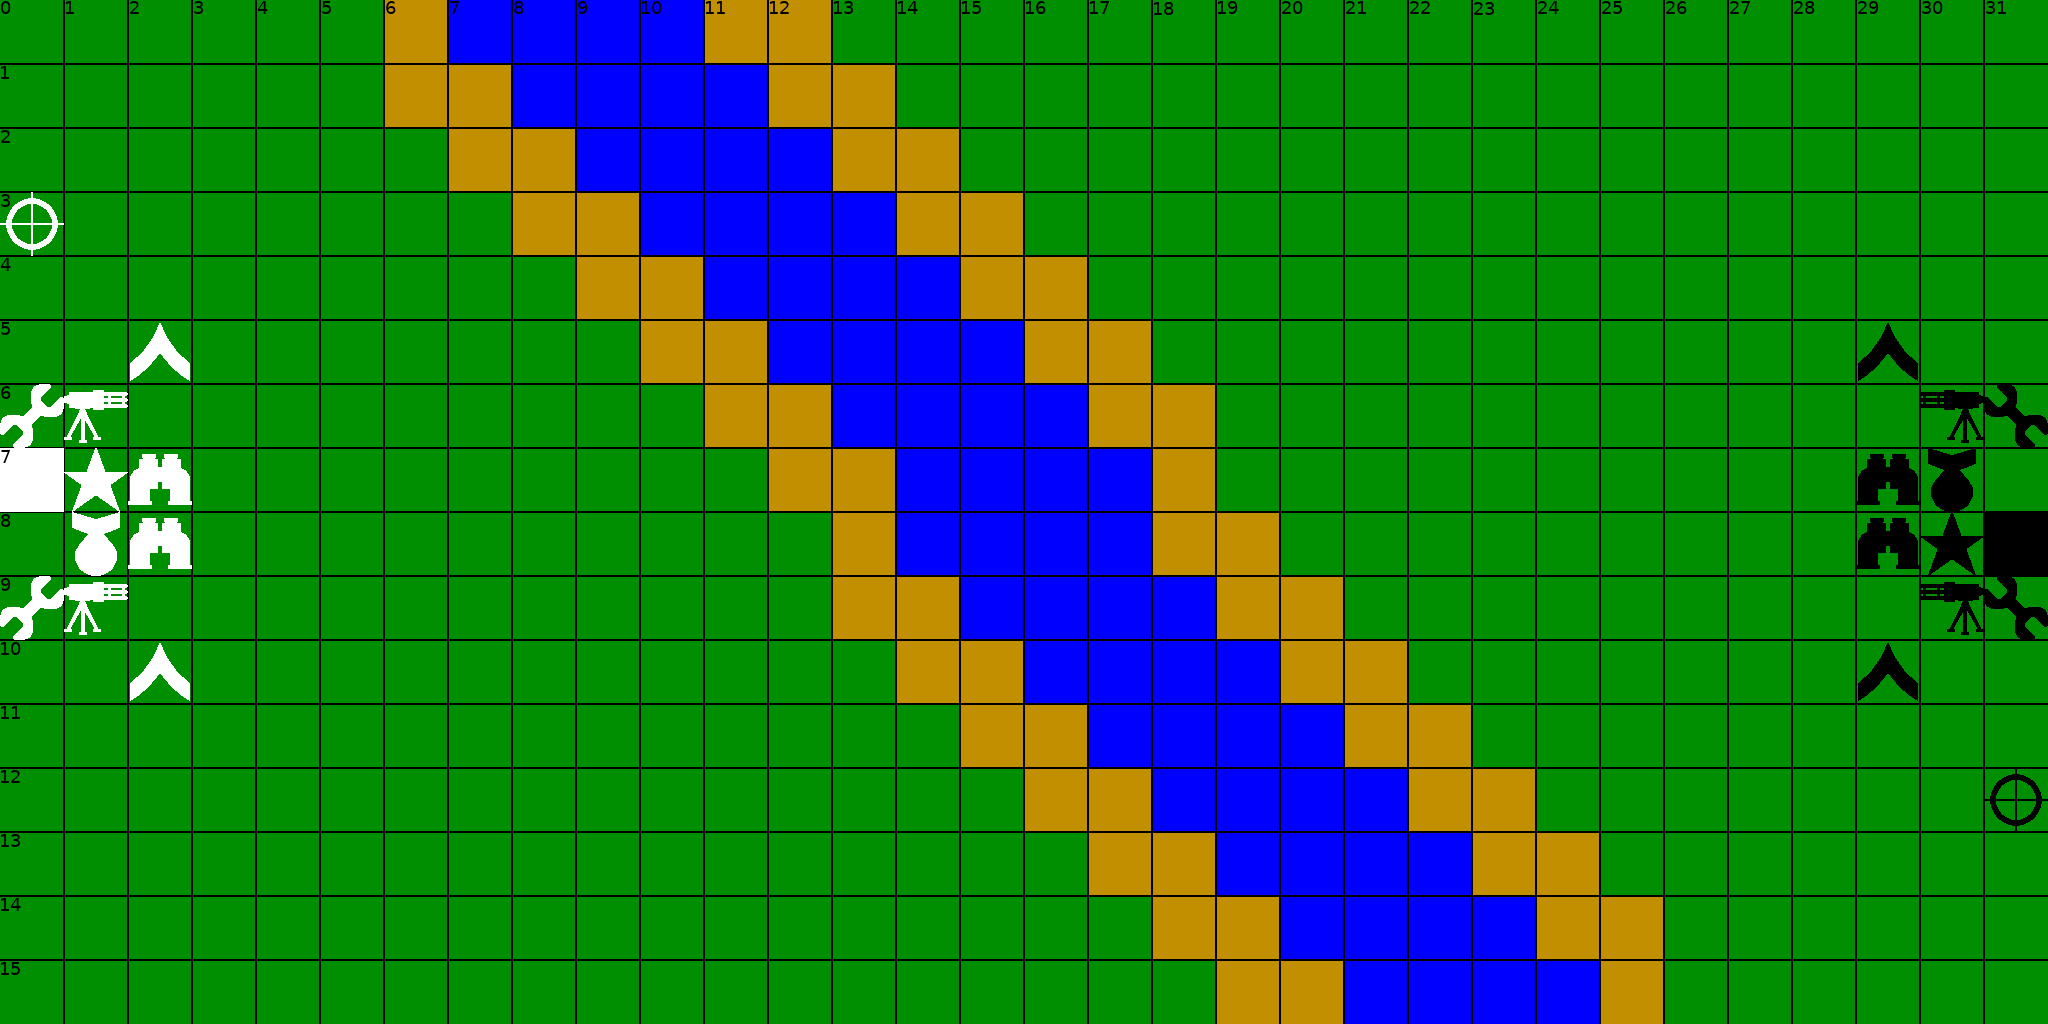
\includegraphics[width=\textwidth]{res/map.png}

Note the prominent river in the middle. It slows movement speed. Additionally
mortars and machineguns cannot setup on it or its banks, nor can snipers remain
camouflaged or engineers build defenses.

Both the beach and the river provide -1 cover, so they are very dangerous for
units to be near.

\section*{Machine Specification}

The virtual environment each team runs on can be defined as follows.

\begin{itemize}[noitemsep]
    \item 11x 1MB main memory (one for each unit)
    \item 11x 1MB direct communications buffer with captain
    \item 1x 1MB direct shared communications buffer
    \item 3x 2KB shared grids (tactical, support, and flag)
    \item 32x registers (some possibly shared)
\end{itemize}

The tables below specify the instructions of each unit. Note that execution
times are in CPU cycles. When two times are listed the shorter is when
successful (cache/branch predictor hit) and the longer is when unsuccessful
(cache/branch predictor miss).

Note that the order of execution within a frame is determined randomly. Whenever
an instruction returns the nearest something, it follows the following route
around the target to find it.

{\centering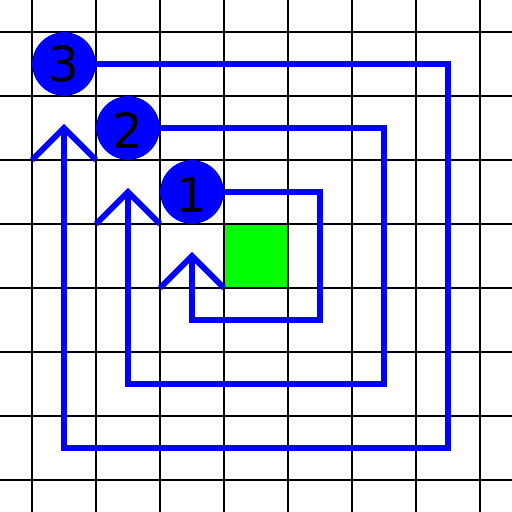
\includegraphics[width=0.5\textwidth]{res/nearest.png}\par}

\subsection*{Registers}

Each unit has 32 32-bit registers. Of these 5 are special purpose, 11 are
general purpose, and 16 are game purpose. They are:

\begin{enumerate}[noitemsep]
    \item R0, this is a read-only register that is always 0. Writing to this
        register has no effect.
    \item R1-R11, these are the general purpose registers.
    \item R12 (IM), this is the immediate register.
    \item R13 (SP), this is the stack pointer.
    \item R14 (LR), this is the link register.
    \item R15 (PC), this is the program counter.
\end{enumerate}

Each unit has 128 assembly instructions. Assembly instructions can take one of 2
forms. Either they will take 3 registers and a 10-bit 2's compliment immediate
or they will take 1 register and a 20-bit unsigned immediate. The register
names in order are A, B, and C.

Register 12 is unique, it is the immediate register. It is a read-only register
that contains the 10-bit signed immediate value.

\subsection*{Floating Point}

Most units have a floating point processor. These operate on IEEE single
precision floating point numbers. The instructions make no distinction between
whether a register is storing an integer or a floating point number.

Note: Depending on hardware, these may be compiled to different 32-bit floating
point standards. A `fully conformant' implementation would use the IEEE
standard. However, do not rely on IEEE representations in your code.

\subsection*{Common}

There are 96 instructions common to all units. These are divided into 3 sets.

The first set is the basic operation set:

\begin{enumerate}[noitemsep]
    \item ADD(1): \texttt{A = B + C}
    \item SUB(1): \texttt{A = B - C}
    \item MUL(4): \texttt{A = B * C}
    \item DIV(8): \texttt{A = B / C}
    \item AND(1): \texttt{A = B \& C}
    \item ORR(1): \texttt{A = B | C}
    \item XOR(1): \texttt{A = B \^{} C}
    \item NAN(1): \texttt{A = ~(B \& C)}
    \item CLZ(1): \texttt{B = clz(A); C = clo(A)}
    \item CNT(1): \texttt{B = popcnt0(A); C = popcnt1(A)}
    \item LSR(1): \texttt{A = B >> C}
    \item LSL(1): \texttt{A = B << C}
    \item ABS(1): \texttt{B = abs(A), C = -abs(A)}
    \item RND(1): \texttt{A, B, C = random}
    \item CMP(1): \texttt{A = (B > C ? 1 : B < C ? -1 : 0)}
    \item JIZ(1/8): \texttt{if A == 0 goto I} (note: assumed taken)
    \item JNZ(1/8): \texttt{if A != 0 goto I} (note: assumed taken)
    \item JGZ(1/8): \texttt{if A > 0 goto I} (note: assumed taken)
    \item JLZ(1/8): \texttt{if A < 0 goto I} (note: assumed taken)
    \item JGE(1/8): \texttt{if A >= 0 goto I} (note: assumed taken)
    \item JLE(1/8): \texttt{if A <= 0 goto I} (note: assumed taken)
    \item BIZ(1/8): \texttt{if A == 0 goto I}
    \item BNZ(1/8): \texttt{if A != 0 goto I}
    \item BGZ(1/8): \texttt{if A > 0 goto I}
    \item BLZ(1/8): \texttt{if A < 0 goto I}
    \item BGE(1/8): \texttt{if A >= 0 goto I}
    \item BLE(1/8): \texttt{if A <= 0 goto I}
    \item BLX(1): \texttt{LR = next PC; goto A + I}
    \item LDR(1/8): \texttt{A = mem[B+C+I]}
    \item STR(1/8): \texttt{mem[B+C+I] = A}
    \item POP(1/8): \texttt{A = mem[++SP]}
    \item PSH(1/8): \texttt{mem[SP--] = A}
\end{enumerate}

The second set is the basic combat set. Here two comma-separated values are X,Y
coordinates. The unit ID's are (SS = sniper-side, FS = far-side):

\begin{tabular}{l|c|c}
    Unit & Friendly ID & Enemy ID \\ \hline
    Captain & 1 & -1 \\ \hline
    Mortar & 2 & -2 \\ \hline
    Sniper & 3 & -3 \\ \hline
    Engineer (SS) & 4 & -4 \\ \hline
    Engineer (FS) & 5 & -5 \\ \hline
    Machinegunner (SS) & 6 & -6 \\ \hline
    Machinegunner (FS) & 7 & -7 \\ \hline
    Scout (SS) & 8 & -8 \\ \hline
    Scout (FS) & 9 & -9 \\ \hline
    Rifleman (SS) & 10 & -10 \\ \hline
    Rifleman (FS) & 11 & -11 \\ \hline
\end{tabular}

As for directions, they are:

\begin{enumerate}[noitemsep]
    \item North
    \item North-East
    \item East
    \item South-East
    \item South
    \item South-West
    \item West
    \item North-West
\end{enumerate}

And terrain types are:

\begin{enumerate}[noitemsep]
    \item Ground
    \item Wire
    \item Cover
    \item Beach
    \item Water
    \item Base
\end{enumerate}

The combat instructions are:

\begin{enumerate}[noitemsep]
    \item WHO(1): \texttt{A = friendly(B,C) ? 1 : -1} (note: 0 if no unit)
    \item WHT(1): \texttt{A = what(B,C)}
    \item QCS(8): \texttt{A = cache size level (B,C)} (note: -1 if no unit)
    \item QCT(8): \texttt{A = cache type level (B,C)} (note: -1 if no unit)
    \item QBP(8): \texttt{A = branch predictor level (B,C)} (note: -1 if no unit)
    \item QCK(8): \texttt{A = clock level (B,C)} (note: -1 if no unit)
    \item GND(1): \texttt{A = ground(B,C)}
    \item WHR(1): \texttt{(B,C) = where(A)} (note: (-1,-1) if unit can't be seen)
    \item DST(4): \texttt{A = distance(here, (B,C))}
    \item CVR(8): \texttt{A = cover to (B,C)}
    \item DED(1): \texttt{B = isDead(A); C = isDead(-A)}
    \item SHT(b+rd+ac): \texttt{shoot(B,C); A = hit?}
    \item DIR(1): \texttt{A = direction to (B,C)}
    \item WLK(8): \texttt{walk in A direction; (B,C) = where(us)}
    \item CRL(64): \texttt{crawl in A direction; (B,C) = where(us)} (note:
        crawling is slower but you can crawl through barbed wire)
    \item SWM(64): \texttt{swim in A direction; (B,C) = where(us)}
    \item CAP(256): \texttt{try to capture base (NOP if not on it)}
    \item RTT(?): \texttt{Retreat to base}
    \item HID(A+I): \texttt{hide for A+I frames} (note: hidden units can only be
        seen by scouts)
    \item SAY(8): \texttt{captain msg[I] = A}
    \item RAD(8): \texttt{A = captain msg[I]}
    \item YEL(16): \texttt{team msg[I] = A}
    \item EAR(16): \texttt{A = team msg[I]}
    \item DIE(0): \texttt{kill this unit}
    \item NRT(4): \texttt{A = what, (B,C) = where first visible unit due north}
    \item NRE(4): \texttt{A = what, (B,C) = where first visible unit due
        north-east}
    \item EST(4): \texttt{A = what, (B,C) = where first visible unit due east}
    \item SOE(4): \texttt{A = what, (B,C) = where first visible unit due
        south-east}
    \item SOT(4): \texttt{A = what, (B,C) = where first visible unit due south}
    \item SOW(4): \texttt{A = what, (B,C) = where first visible unit due
        south-west}
    \item WST(4): \texttt{A = what, (B,C) = where first visible unit due west}
    \item NRW(4): \texttt{A = what, (B,C) = where first visible unit due
        north-west}
\end{enumerate}

The third set are the upgrade commands. They are:

\begin{enumerate}[noitemsep]
    \item WCS(1): \texttt{A = my cache size level}
    \item WCT(1): \texttt{A = my cache type level}
    \item WBP(1): \texttt{A = my branch predictor level}
    \item WCL(1): \texttt{A = my clock level}
    \item TCS(1): \texttt{A = cache size level of teammate I}
    \item TCT(1): \texttt{A = cache type level of teammate I}
    \item TBP(1): \texttt{A = branch predictor level of teammate I}
    \item TCL(1): \texttt{A = clock level of teammate I}
    \item PNT(1): \texttt{A = team resources}
    \item CCS(1): \texttt{A = next cache size level cost}
    \item CCT(1): \texttt{A = next cache type level cost}
    \item CBP(1): \texttt{A = next branch predictor level cost}
    \item CCL(1): \texttt{A = next clock level cost}
    \item UCS(1): \texttt{upgrade cache size (A = success?1:0)}
    \item UCT(1): \texttt{upgrade cache type (A = success?1:0)}
    \item UBP(1): \texttt{upgrade branch predictor (A = success?1:0)}
    \item UCL(1): \texttt{upgrade clock (A = success?1:0)}
    \item DCS(1): \texttt{downgrade cache size (A = success?1:0)}
    \item DCT(1): \texttt{downgrade cache type (A = success?1:0)}
    \item DBP(1): \texttt{downgrade branch predictor (A = success?1:0)}
    \item DCL(1): \texttt{downgrade clock (A = success?1:0)}
    \item MCS(1): \texttt{max cache size (A = success?1:0)}
    \item MCT(1): \texttt{max cache type (A = success?1:0)}
    \item MBP(1): \texttt{max branch predictor (A = success?1:0)}
    \item MCL(1): \texttt{max clock (A = success?1:0)}
    \item RCS(1): \texttt{reset cache size (A = success?1:0)}
    \item RCT(1): \texttt{reset cache type (A = success?1:0)}
    \item RBP(1): \texttt{reset branch predictor (A = success?1:0)}
    \item RCL(1): \texttt{reset clock (A = success?1:0)}
    \item TIM(1): \texttt{A = universal clock, B = my relative clock, C = my
        team's relative clock}
    \item DLY(1): \texttt{delay 1 universal tick}
    \item ADV(4): \texttt{next operation takes 1 less universal tick}
\end{enumerate}

\subsection*{Captain}

The captain's special registers are:

\begin{enumerate}[noitemsep]
    \item Team resources
    \item Enemy resources
    \item Nearest Ally X
    \item Nearest Ally Y
    \item Mortar alive? (1 = ours, 2 = theirs, 3 = both, 0 = neither)
    \item Sniper alive?
    \item Engineer (SS) alive?
    \item Engineer (FS) alive?
    \item Machinegunner (SS) alive?
    \item Machinegunner (FS) alive?
    \item Scout (SS) alive?
    \item Scout (FS) alive?
    \item Rifleman (SS) alive?
    \item Rifleman (FS) alive?
    \item Bomb requests
    \item Air requests
\end{enumerate}

The captain's special abilities are:

\begin{enumerate}[noitemsep]
    \item ASK(4): \texttt{Gain 1 resource}
    \item PLZ(8): \texttt{Gain 4 resources}
    \item BEG(16): \texttt{Gain 16 resources}
    \item GVL(32): \texttt{Gain 64 resources}
    \item KMK(1): \texttt{Die and gain 1024 resources}
    \item SAC(1): \texttt{Kill friendly A and gain 1024 resources}
    \item BOM(256): \texttt{Kill any unit in the water} (costs 128 RP)
    \item AIR(128): \texttt{Kill any unit on the nearest beach} (costs 64 RP)
    \item SUM(?): \texttt{Summon friendly A} (note: summoned units pause
        execution and move towards captain as fast as possible until they
        are adjacent)
    \item HAK(16): \texttt{enemy team msg[I] = A}
    \item EMP(256): \texttt{enemy team msg[all] = 0}
    \item ALL(1): \texttt{all msg[I] = A}
    \item RMT(1): \texttt{A = mortar msg[I]}
    \item RSN(1): \texttt{A = sniper msg[I]}
    \item RES(1): \texttt{A = engineer (SS) msg[I]}
    \item REF(1): \texttt{A = engineer (FS) msg[I]}
    \item RMS(1): \texttt{A = machinegunner (SS) msg[I]}
    \item RMF(1): \texttt{A = machinegunner (FS) msg[I]}
    \item RSS(1): \texttt{A = scout (SS) msg[I]}
    \item RSF(1): \texttt{A = scout (FS) msg[I]}
    \item RRS(1): \texttt{A = rifleman (SS) msg[I]}
    \item RRF(1): \texttt{A = rifleman (FS) msg[I]}
    \item WMT(1): \texttt{mortar msg[I] = A}
    \item WSN(1): \texttt{sniper msg[I] = A}
    \item WES(1): \texttt{engineer (SS) msg[I] = A}
    \item WEF(1): \texttt{engineer (FS) msg[I] = A}
    \item WMS(1): \texttt{machinegunner (SS) msg[I] = A}
    \item WMF(1): \texttt{machinegunner (FS) msg[I] = A}
    \item WSS(1): \texttt{scout (SS) msg[I] = A}
    \item WSF(1): \texttt{scout (FS) msg[I] = A}
    \item WRS(1): \texttt{rifleman (SS) msg[I] = A}
    \item WRF(1): \texttt{rifleman (FS) msg[I] = A}
\end{enumerate}

\subsection*{Mortar}

The mortar's special registers are:

\begin{enumerate}[noitemsep]
    \item Bomb request X
    \item Bomb request Y
    \item Enemy Scout (SS) X
    \item Enemy Scout (SS) Y
    \item Enemy Scout (FS) X
    \item Enemy Scout (FS) Y
    \item Allied Captain X
    \item Allied Sniper X
    \item Allied Engineer (SS) X
    \item Allied Engineer (FS) X
    \item Allied Machinegunner (SS) X
    \item Allied Machinegunner (FS) X
    \item Allied Scout (SS) X
    \item Allied Scout (FS) X
    \item Allied Rifleman (SS) X
    \item Allied Rifleman (FS) X
\end{enumerate}

The mortar's special abilities are:

\begin{enumerate}[noitemsep]
    \item WTG(4): \texttt{tactical grid[B,C] = A}
    \item RTG(4): \texttt{A = tactical grid[B,C]}
    \item WSG(4): \texttt{support grid[B,C] = A}
    \item RSG(4): \texttt{A = support grid[B,C]}
    \item WFG(4): \texttt{flag grid[B,C] = A}
    \item RFG(4): \texttt{A = flag grid[B,C]}
    \item ITF(8): \texttt{A = float(I)}
    \item FAD(8): \texttt{A = float(B) + float(C)}
    \item FSU(8): \texttt{A = float(B) - float(C)}
    \item FMU(32): \texttt{A = float(B) * float(C)}
    \item FDV(64): \texttt{A = float(B) / float(C)}
    \item CEL(8): \texttt{A = ceil(A)}
    \item FLR(8): \texttt{A = floor(A)}
    \item SIN(64): \texttt{A = sin(A)}
    \item COS(64): \texttt{A = cos(A)}
    \item TAN(64): \texttt{A = tan(A)}
    \item POW(64): \texttt{A = float(B) \^{} float(C)}
    \item ASN(64): \texttt{A = asin(A)}
    \item ACS(64): \texttt{A = acos(A)}
    \item ATN(64): \texttt{A = atan(A)}
    \item LOG(64): \texttt{A = log base float(C) of float(B)}
    \item FCP(8): \texttt{A = floatcmp(B,C)}
    \item MLE(16): \texttt{melee around current position}
    \item SET(128): \texttt{setup weapon}
    \item CSS(8): \texttt{ask engineer (SS) for cover at (B,C); A = success?1:0}
    \item CFS(8): \texttt{ask engineer (FS) for cover at (B,C); A = success?1:0}
    \item WSS(8): \texttt{ask engineer (SS) for wire at (B,C); A = success?1:0}
    \item WFS(8): \texttt{ask engineer (FS) for wire at (B,C); A = success?1:0}
    \item BOM(8): \texttt{ask captain to bomb I times; A = success?1:0}
    \item AIR(8): \texttt{ask captain to air I times; A = success?1:0}
    \item GUP(128): \texttt{unsetup weapon}
    \item SUP(8): \texttt{ask riflemen for support}
\end{enumerate}

\subsection*{Sniper}

The sniper's special registers are:

\begin{enumerate}[noitemsep]
    \item Camouflage status (1 = hidden, 0 = not)
    \item Enemy count within 1 square
    \item Enemy count within 2 squares
    \item Enemy count within 3 squares
    \item Read-only direct-link register with Scout (SS)
    \item Read-only direct-link register with Scout (SS)
    \item Read-only direct-link register with Scout (FS)
    \item Read-only direct-link register with Scout (FS)
    \item Write-only direct-link register with Scout (SS)
    \item Write-only direct-link register with Scout (SS)
    \item Write-only direct-link register with Scout (FS)
    \item Write-only direct-link register with Scout (FS)
    \item Nearest enemy X
    \item Nearest enemy Y
    \item Enemy captain X
    \item Enemy captain Y
\end{enumerate}

The sniper's special abilities are:

\begin{enumerate}[noitemsep]
    \item CAM(64): \texttt{enter camouflage}
    \item UNC(1): \texttt{exit camouflage}
    \item HIP(4+4r+16c): \texttt{hip shot(B,C); A = hit?} (costs 64 RP)
    \item NMR(1): \texttt{(B,C) = next mortar hit, A = universal ticks until}
        (note: all -1 if none in progress)
    \item IST(8): \texttt{A = targeter of (B,C)}
    \item TGT(16): \texttt{(B,C) = target of unit A} (note: (-1,-1) if none)
    \item ITF(8): \texttt{A = float(I)}
    \item FAD(8): \texttt{A = float(B) + float(C)}
    \item FSU(8): \texttt{A = float(B) - float(C)}
    \item FMU(32): \texttt{A = float(B) * float(C)}
    \item FDV(64): \texttt{A = float(B) / float(C)}
    \item CEL(8): \texttt{A = ceil(A)}
    \item FLR(8): \texttt{A = floor(A)}
    \item SIN(64): \texttt{A = sin(A)}
    \item COS(64): \texttt{A = cos(A)}
    \item TAN(64): \texttt{A = tan(A)}
    \item POW(64): \texttt{A = float(B) \^{} float(C)}
    \item ASN(64): \texttt{A = asin(A)}
    \item ACS(64): \texttt{A = acos(A)}
    \item ATN(64): \texttt{A = atan(A)}
    \item LOG(64): \texttt{A = log base float(C) of float(B)}
    \item FCP(8): \texttt{A = floatcmp(B,C)}
    \item LIE(64): \texttt{lie down}
    \item GUP(64): \texttt{get up}
    \item CSS(8): \texttt{ask engineer (SS) for cover at (B,C); A = success?1:0}
    \item CFS(8): \texttt{ask engineer (FS) for cover at (B,C); A = success?1:0}
    \item WSS(8): \texttt{ask engineer (SS) for wire at (B,C); A = success?1:0}
    \item WFS(8): \texttt{ask engineer (FS) for wire at (B,C); A = success?1:0}
    \item BOM(8): \texttt{ask captain to bomb I times; A = success?1:0}
    \item AIR(8): \texttt{ask captain to air I times; A = success?1:0}
    \item MOR(8): \texttt{ask mortar to bomb (B,C); A = success?1:0}
    \item SUP(8): \texttt{ask riflemen for support}
\end{enumerate}

\subsection*{Engineer}

The engineer's special registers are:

\begin{enumerate}[noitemsep]
    \item Cover request X
    \item Cover request Y
    \item Wire request X
    \item Wire request Y
    \item Nearest cover X
    \item Nearest cover Y
    \item Nearest wire X
    \item Nearest wire Y
    \item Nearest ally X
    \item Nearest ally Y
    \item Nearest enemy X
    \item Nearest enemy Y
    \item Nearest river X
    \item Nearest river Y
    \item Distance to base
    \item Distance to enemy base
\end{enumerate}

The engineer's special abilities are:

\begin{enumerate}[noitemsep]
    \item WIR(8): \texttt{plant wire in direction A}
    \item CUT(8): \texttt{cut wire in direction A}
    \item SND(8): \texttt{plant cover in direction A}
    \item DIG(8): \texttt{remove cover in direction A}
    \item WFG(4): \texttt{flag grid[B,C] = A}
    \item RFG(4): \texttt{A = flag grid[B,C]}
    \item ITF(8): \texttt{A = float(I)}
    \item FAD(8): \texttt{A = float(B) + float(C)}
    \item FSU(8): \texttt{A = float(B) - float(C)}
    \item FMU(32): \texttt{A = float(B) * float(C)}
    \item FDV(64): \texttt{A = float(B) / float(C)}
    \item CEL(8): \texttt{A = ceil(A)}
    \item FLR(8): \texttt{A = floor(A)}
    \item SIN(64): \texttt{A = sin(A)}
    \item COS(64): \texttt{A = cos(A)}
    \item TAN(64): \texttt{A = tan(A)}
    \item POW(64): \texttt{A = float(B) \^{} float(C)}
    \item ASN(64): \texttt{A = asin(A)}
    \item ACS(64): \texttt{A = acos(A)}
    \item ATN(64): \texttt{A = atan(A)}
    \item LOG(64): \texttt{A = log base float(C) of float(B)}
    \item FCP(8): \texttt{A = floatcmp(B,C)}
    \item LIE(64): \texttt{lie down}
    \item GUP(64): \texttt{get up}
    \item CSS(8): \texttt{ask engineer (SS) for cover at (B,C); A = success?1:0}
    \item CFS(8): \texttt{ask engineer (FS) for cover at (B,C); A = success?1:0}
    \item WSS(8): \texttt{ask engineer (SS) for wire at (B,C); A = success?1:0}
    \item WFS(8): \texttt{ask engineer (FS) for wire at (B,C); A = success?1:0}
    \item BOM(8): \texttt{ask captain to bomb I times; A = success?1:0}
    \item AIR(8): \texttt{ask captain to air I times; A = success?1:0}
    \item MOR(8): \texttt{ask mortar to bomb (B,C); A = success?1:0}
    \item SUP(8): \texttt{ask riflemen for support}
\end{enumerate}

\subsection*{Machinegunner}

The machinegunner's special registers are:

\begin{enumerate}[noitemsep]
    \item Setup status (1 = setup, 0 = holding)
    \item Nearest enemy X
    \item Nearest enemy Y
    \item Fire time to nearest enemy
    \item Number of enemy units adjacent to self
    \item Number of enemy units within 2 squares of self
    \item Number of enemy units within 3 squares of self
    \item Number of enemy units within 4 squares of self
    \item Number of enemy units within 5 squares of self
    \item Number of enemy units within 6 squares of self
    \item Number of allied units adjacent to self
    \item Number of allied units within 2 squares of self
    \item Number of allied units within 3 squares of self
    \item Number of allied units within 4 squares of self
    \item Number of allied units within 5 squares of self
    \item Number of allied units within 6 squares of self
\end{enumerate}

The machinegunner's special abilities are:

\begin{enumerate}[noitemsep]
    \item SET(128) \texttt{setup weapon}
    \item GUP(128) \texttt{unsetup weapon}
    \item WSG(4): \texttt{support grid[B,C] = A}
    \item RSG(4): \texttt{A = support grid[B,C]}
    \item WFG(4): \texttt{flag grid[B,C] = A}
    \item RFG(4): \texttt{A = flag grid[B,C]}
    \item ITF(8): \texttt{A = float(I)}
    \item FAD(8): \texttt{A = float(B) + float(C)}
    \item FSU(8): \texttt{A = float(B) - float(C)}
    \item FMU(32): \texttt{A = float(B) * float(C)}
    \item FDV(64): \texttt{A = float(B) / float(C)}
    \item CEL(8): \texttt{A = ceil(A)}
    \item FLR(8): \texttt{A = floor(A)}
    \item SIN(64): \texttt{A = sin(A)}
    \item COS(64): \texttt{A = cos(A)}
    \item TAN(64): \texttt{A = tan(A)}
    \item POW(64): \texttt{A = float(B) \^{} float(C)}
    \item ASN(64): \texttt{A = asin(A)}
    \item ACS(64): \texttt{A = acos(A)}
    \item ATN(64): \texttt{A = atan(A)}
    \item LOG(64): \texttt{A = log base float(C) of float(B)}
    \item FCP(8): \texttt{A = floatcmp(B,C)}
    \item MLE(16): \texttt{melee around current position}
    \item MLF(4): \texttt{melee in direction A}
    \item CSS(8): \texttt{ask engineer (SS) for cover at (B,C); A = success?1:0}
    \item CFS(8): \texttt{ask engineer (FS) for cover at (B,C); A = success?1:0}
    \item WSS(8): \texttt{ask engineer (SS) for wire at (B,C); A = success?1:0}
    \item WFS(8): \texttt{ask engineer (FS) for wire at (B,C); A = success?1:0}
    \item BOM(8): \texttt{ask captain to bomb I times; A = success?1:0}
    \item AIR(8): \texttt{ask captain to air I times; A = success?1:0}
    \item MOR(8): \texttt{ask mortar to bomb (B,C); A = success?1:0}
    \item SUP(8): \texttt{ask riflemen for support}
\end{enumerate}

\subsection*{Scout}

The scout's special registers are:

\begin{enumerate}[noitemsep]
    \item Sniper camouflage status
    \item Enemy sniper camouflage status
    \item Write-only direct-link register with Sniper
    \item Write-only direct-link register with Sniper
    \item Read-only direct-link register with Sniper
    \item Read-only direct-link register with Sniper
    \item Nearest enemy X
    \item Nearest enemy Y
    \item Second nearest enemy X
    \item Second nearest enemy Y
    \item Third nearest enemy X
    \item Third nearest enemy Y
    \item Fourth nearest enemy X
    \item Fourth nearest enemy Y
    \item Fifth nearest enemy X
    \item Fifth nearest enemy Y
\end{enumerate}

The scout's special abilities are:

\begin{enumerate}[noitemsep]
    \item RUN(1): \texttt{run in A direction; (B,C) = where(us)}
    \item HIT(16): \texttt{hit in A direction; B = hit?} (note: this is slower
        than a point-blank shot, but is free)
    \item WSG(4): \texttt{support grid[B,C] = A}
    \item RSG(4): \texttt{A = support grid[B,C]}
    \item WFG(4): \texttt{flag grid[B,C] = A}
    \item RFG(4): \texttt{A = flag grid[B,C]}
    \item ITF(8): \texttt{A = float(I)}
    \item FAD(8): \texttt{A = float(B) + float(C)}
    \item FSU(8): \texttt{A = float(B) - float(C)}
    \item FMU(32): \texttt{A = float(B) * float(C)}
    \item FDV(64): \texttt{A = float(B) / float(C)}
    \item CEL(8): \texttt{A = ceil(A)}
    \item FLR(8): \texttt{A = floor(A)}
    \item SIN(64): \texttt{A = sin(A)}
    \item COS(64): \texttt{A = cos(A)}
    \item TAN(64): \texttt{A = tan(A)}
    \item POW(64): \texttt{A = float(B) \^{} float(C)}
    \item ASN(64): \texttt{A = asin(A)}
    \item ACS(64): \texttt{A = acos(A)}
    \item ATN(64): \texttt{A = atan(A)}
    \item LOG(64): \texttt{A = log base float(C) of float(B)}
    \item FCP(8): \texttt{A = floatcmp(B,C)}
    \item LIE(64): \texttt{lie down}
    \item GUP(64): \texttt{get up}
    \item CSS(8): \texttt{ask engineer (SS) for cover at (B,C); A = success?1:0}
    \item CFS(8): \texttt{ask engineer (FS) for cover at (B,C); A = success?1:0}
    \item WSS(8): \texttt{ask engineer (SS) for wire at (B,C); A = success?1:0}
    \item WFS(8): \texttt{ask engineer (FS) for wire at (B,C); A = success?1:0}
    \item BOM(8): \texttt{ask captain to bomb I times; A = success?1:0}
    \item AIR(8): \texttt{ask captain to air I times; A = success?1:0}
    \item MOR(8): \texttt{ask mortar to bomb (B,C); A = success?1:0}
    \item SUP(8): \texttt{ask riflemen for support}
\end{enumerate}

\subsection*{Rifleman}

The rifleman's special registers are:

\begin{enumerate}[noitemsep]
    \item Last support X
    \item Last support Y
    \item Last enemy support X
    \item Last enemy support Y
    \item Number of enemy units adjacent to self
    \item Number of enemy units within 2 squares of self
    \item Number of enemy units within 3 squares of self
    \item Number of enemy units within 4 squares of self
    \item Number of enemy units within 5 squares of self
    \item Number of enemy units within 6 squares of self
    \item Number of allied units adjacent to self
    \item Number of allied units within 2 squares of self
    \item Number of allied units within 3 squares of self
    \item Number of allied units within 4 squares of self
    \item Number of allied units within 5 squares of self
    \item Number of allied units within 6 squares of self
\end{enumerate}

The rifleman's special abilities are:

\begin{enumerate}[noitemsep]
    \item WTG(4): \texttt{tactical grid[B,C] = A}
    \item RTG(4): \texttt{A = tactical grid[B,C]}
    \item WSG(4): \texttt{support grid[B,C] = A}
    \item RSG(4): \texttt{A = support grid[B,C]}
    \item WFG(4): \texttt{flag grid[B,C] = A}
    \item RFG(4): \texttt{A = flag grid[B,C]}
    \item ITF(8): \texttt{A = float(I)}
    \item FAD(8): \texttt{A = float(B) + float(C)}
    \item FSU(8): \texttt{A = float(B) - float(C)}
    \item FMU(32): \texttt{A = float(B) * float(C)}
    \item FDV(64): \texttt{A = float(B) / float(C)}
    \item CEL(8): \texttt{A = ceil(A)}
    \item FLR(8): \texttt{A = floor(A)}
    \item SIN(64): \texttt{A = sin(A)}
    \item COS(64): \texttt{A = cos(A)}
    \item TAN(64): \texttt{A = tan(A)}
    \item POW(64): \texttt{A = float(B) \^{} float(C)}
    \item ASN(64): \texttt{A = asin(A)}
    \item ACS(64): \texttt{A = acos(A)}
    \item ATN(64): \texttt{A = atan(A)}
    \item LOG(64): \texttt{A = log base float(C) of float(B)}
    \item FCP(8): \texttt{A = floatcmp(B,C)}
    \item LIE(64): \texttt{lie down}
    \item GUP(64): \texttt{get up}
    \item CSS(8): \texttt{ask engineer (SS) for cover at (B,C); A = success?1:0}
    \item CFS(8): \texttt{ask engineer (FS) for cover at (B,C); A = success?1:0}
    \item WSS(8): \texttt{ask engineer (SS) for wire at (B,C); A = success?1:0}
    \item WFS(8): \texttt{ask engineer (FS) for wire at (B,C); A = success?1:0}
    \item BOM(8): \texttt{ask captain to bomb I times; A = success?1:0}
    \item AIR(8): \texttt{ask captain to air I times; A = success?1:0}
    \item MOR(8): \texttt{ask mortar to bomb (B,C); A = success?1:0}
    \item SUP(8): \texttt{ask riflemen for support}
\end{enumerate}

\section*{Machine Language}

The machine language runs each 4-byte instruction one at a time. They are
encoded as:

\texttt{NNNNNNNA AAAABBBB BCCCCCII IIIIIIII}

or

\texttt{NNNNNNNA AAAAIIII IIIIIIII IIIIIIII}

\subsection*{Debug Mode}

\textit{Coming soon!}

In debug mode the DIE command, while still taking no time, will not kill the
unit, but rather print the null-terminated ASCII string of its immediate value
to standard output. In order to facilitate this, the bits of the A register are
used for extended memory access.

\section*{Assembly Language}

In order to facilitate development, this game comes with an assembler. All
directives are 3-letter case-insensitive strings. Every command compiles to its
binary representation. Arguments are separated by commas, immediates can be
written directly as C-style integers.  The comment character is the semi-colon.

Absolute labels are created by postfixing an identifier with a colon. The
identifier of any label is a valid large immediate value. Additionally any
number of words can be added to or subtracted from a label. The special label
`.' represents the current address.

Any line beginning with \verb|#| marks the raw inclusion of another file. The
rest of the line is treated as a path to the file whose contents to dump.

The special directives: \texttt{!captain}, \texttt{!mortar}, \texttt{!sniper},
\texttt{!engineer\_ss}, \texttt{!engineer\_fs}, \texttt{!mg\_ss},
\texttt{!mg\_fs}, \texttt{!scout\_ss}, \texttt{!scout\_fs},
\texttt{!rifleman\_ss}, and \texttt{!rifleman\_fs} indicate a switch to the
associated unit's code. In order to successfully assemble, a source file must
include all of these sections (though possibly via includes).

Raw code substitution aliases may be defined using the equal sign. For example
it is useful to define \texttt{PC = r15}. These definitions must be the only
content on their lines other than an optional comment. The left hand side must
be exactly an identifier, the right hand side can be anything -- any comment
will be stripped and the identifier replaced with the right hand side verbatim.

Finally the special directive \texttt{RAW} embeds the following 32-bit signed
integer directly into memory.

An EBNF description of the assembly language is thus:

\begin{verbatim}program = line*
line = (memory_word | assignment)? comment?
assignment = identifier "=" any-symbol+
memory_word = section? label* data | include
section = "!" section-name whitespace
label = identifier ":"
data = directive whitespace register "," register "," register |
       directive whitespace register "," immediate |
       directive whitespace immediate
register = register-name | immediate
immediate = c-style-literal | identifier
register-name = "r0" | "r1" | ... | "r31"
\end{verbatim}

\end{document}
